\documentclass{beamer}
\usepackage{ctex, hyperref}
\usepackage[T1]{fontenc}

% other packages
\usepackage{latexsym,amsmath,xcolor,multicol,booktabs,calligra}
\usepackage{graphicx,pstricks,listings,stackengine,svg}
\usepackage{tikz}
\usepackage{caption} % 添加caption宏包

% 设置caption标签为"Fig."
\captionsetup[figure]{name=Fig.}
\captionsetup[table]{name=Tab.}
\captionsetup{font=footnotesize}

\newcommand\Background{%
\begin{tikzpicture}[remember picture,overlay]
\node[inner sep=0pt,outer sep=0pt,opacity=0.5]
  at (current page.center)
  {
\includegraphics[height=0.8\paperheight]{pic/logo_faint.png}};
\end{tikzpicture}%
}

\author[陆知雨]{E Ash, M Morelli, M Vannoni}
\title{Journal Report}
\subtitle{More Laws, More Growth? Evidence from
US States}
\institute[中国财政发展协同创新中心]{Journal of Political Economy 133.5 (2025)}%在`[]`中打入会在下栏中显示
\date{DOI:10.1086/734874}
\usepackage{cufe}

% defs
\def\cmd#1{\texttt{\color{red}\footnotesize $\backslash$#1}}
\def\env#1{\texttt{\color{blue}\footnotesize #1}}
\definecolor{deepblue}{rgb}{0,0,0.5}
\definecolor{deepred}{rgb}{0.6,0,0}
\definecolor{deepgreen}{rgb}{0,0.5,0}
\definecolor{halfgray}{gray}{0.55}

\lstset{
    basicstyle=\ttfamily\small,
    keywordstyle=\bfseries\color{deepblue},
    emphstyle=\ttfamily\color{deepred},    % Custom highlighting style
    stringstyle=\color{deepgreen},
    numbers=left,
    numberstyle=\small\color{halfgray},
    rulesepcolor=\color{red!20!green!20!blue!20},
    frame=shadowbox,
}


\begin{document}


\begin{frame}
    \Background
    \titlepage
\end{frame}

\section{Introduction}

\begin{frame}
    \frametitle{Background}
    \begin{itemize}
        \item Empirical evidence shows that states with larger, more complex legal systems also tend to have larger, more productive economies.
        \begin{figure}[htbp]
            \centering
            \begin{minipage}{0.45\textwidth}
                \centering
                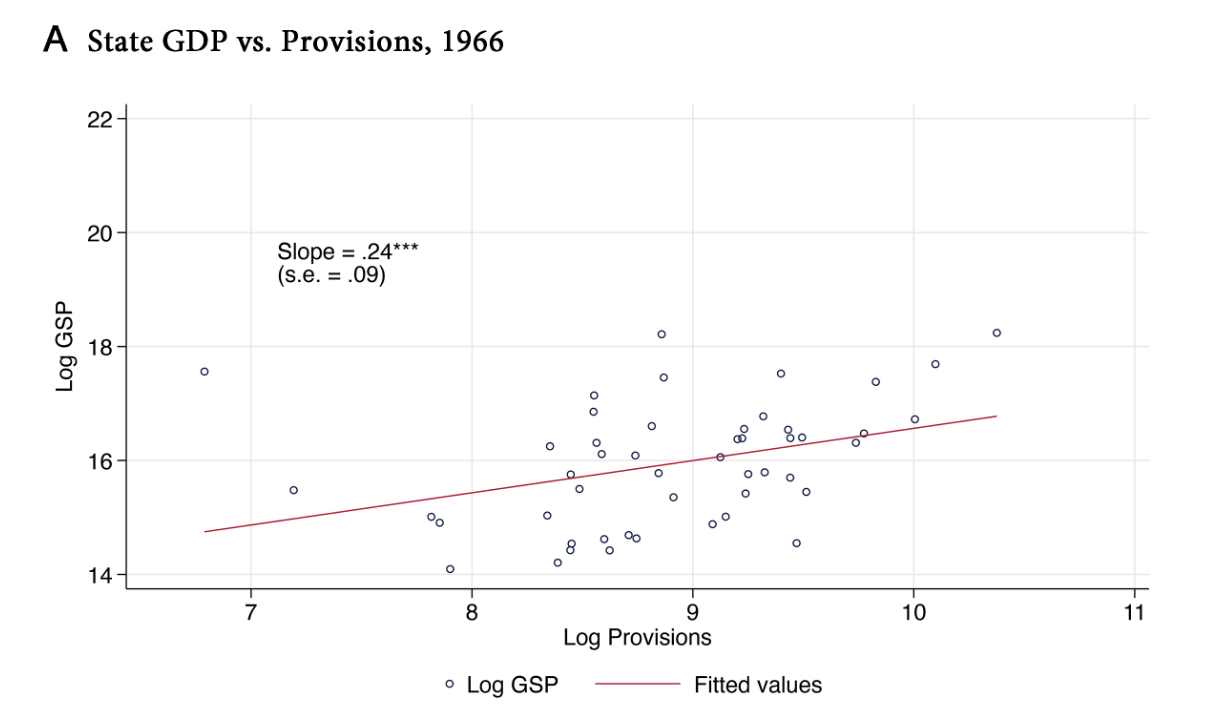
\includegraphics[width=\textwidth]{pic/fig1.png}
            \end{minipage}
            \hfill
            \begin{minipage}{0.45\textwidth}
                \centering
                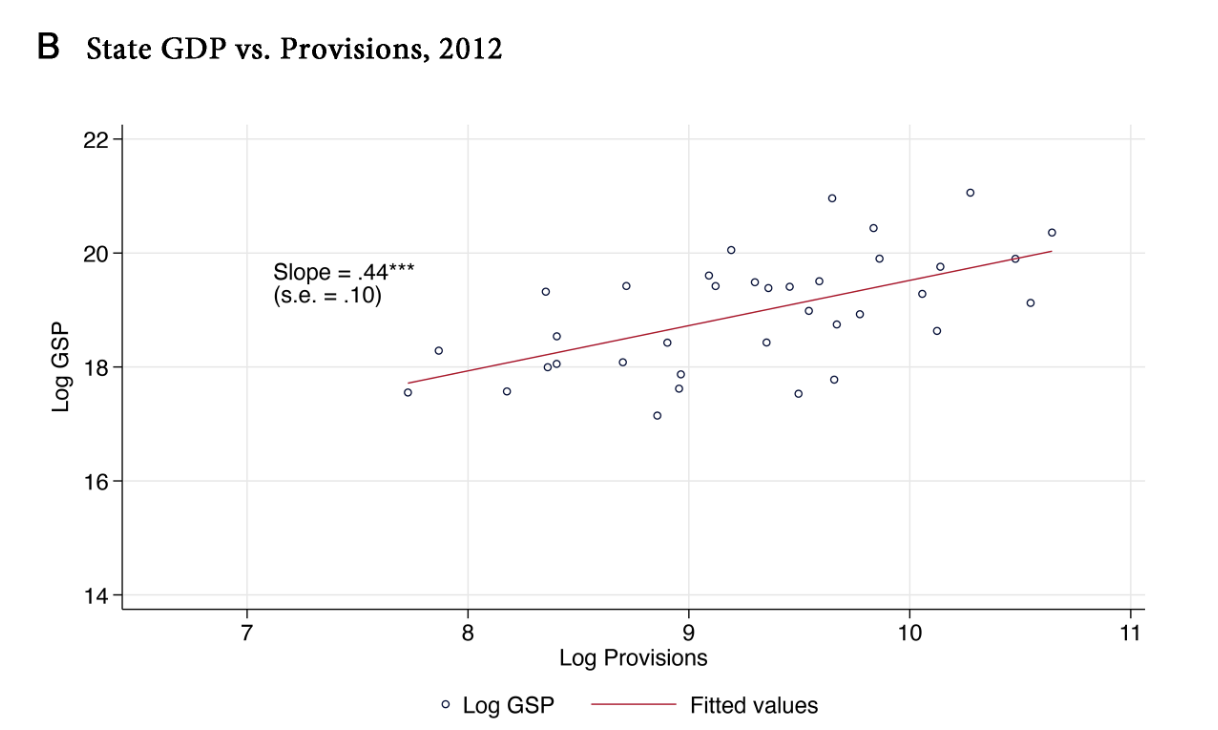
\includegraphics[width=\textwidth]{pic/fig2.png}
            \end{minipage}
            \caption{State GDP and legislative output, 1966 and 2012}
        \end{figure}

        \item \textbf{Whether these correlations reflect causal links?}
    \end{itemize}
\end{frame}

\begin{frame}
    \frametitle{Literature Review and Key Findings} 
\begin{columns}[T] 

\begin{column}{0.5\textwidth}
    \begin{block}{\small Legislation as Catalyst}
        {\footnotesize
        \begin{itemize}
            \item Institutions born from law are essential for markets to operate efficiently and thus \textbf{directly cause economic growth} (Dam 2007).
            \item Furthermore, a detailed and reliable “legislative contract” provides the certainty needed to \textbf{unleash investment} and drive progress (Williamson 1979; Hart and Moore 1988).
        \end{itemize}
        }
    \end{block}
\end{column}

\begin{column}{0.5\textwidth}
    \begin{block}{\small Legislation as Impediment}
        {\footnotesize
        \begin{itemize}
            \item Legislation can potentially hinder economic progress.
            \item Laws might primarily \textbf{serve special interest groups} (Grossman and Helpman 2001).
            \item Even with well-intentioned legislators, excessive lawmaking can impose \textbf{compliance costs} (Niskanen 1971; Botero et al. 2004).
        \end{itemize}
        }
    \end{block}
\end{column}
\end{columns}

\vspace{-0.3cm} % Reduce space between columns and author block

\begin{block}{\small Proposition and Empirical Findings}
    {\footnotesize
    \textbf{ Whether and how laws impact the economy?}

    \textbf{Key Finding:} Increasing legal detail leads to more growth by reducing legal uncertainty.
    }
\end{block}

\end{frame}

\begin{frame}{Big Picture}
\begin{figure}[htbp]
    \centering
    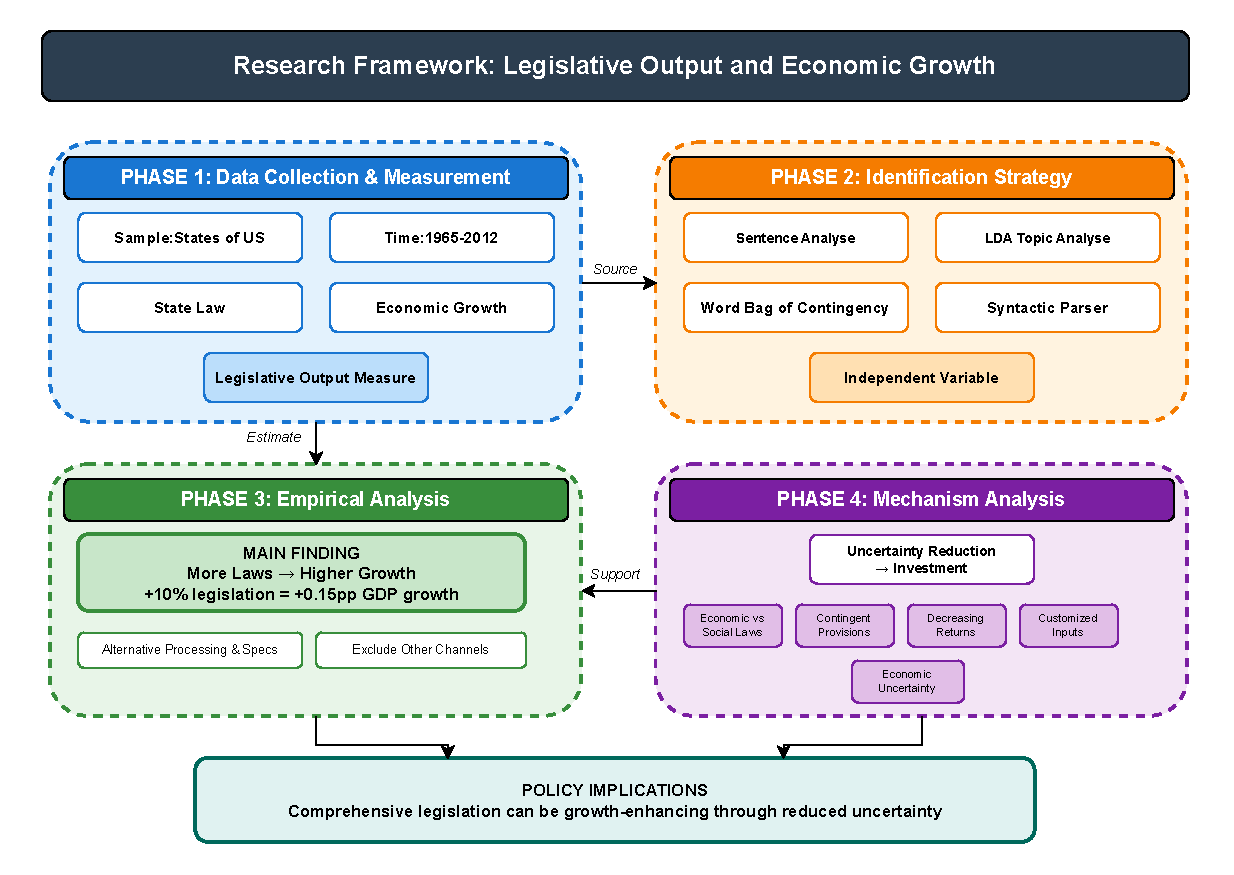
\includegraphics[width=0.95\textwidth]{pic/fig3.pdf}
        \caption{Big Picture}
\end{figure}
\end{frame}

\section{Data and Variable} 
\begin{frame}
    \frametitle{Main Variables}
    {\small % 使用更小的字体
    \begin{itemize}
        \item \textbf{Data Scope:} The dataset includes 50 US states, covering the period from 1965 to 2012, with observations at 2-year intervals.
        \item \textbf{Dependent Variable:} Economic growth
        \begin{itemize}
            \item \textbf{Source:} Bureau of Economic Analysis Regional Accounts, County Business Patterns, Klarner (2013), and Ujhelyi (2014)
            \item \textbf{Measurement:} Change in log per capita GSP in state s between year $t-2$ and year $t$
        \end{itemize}
        \item \textbf{Independent Variable:} State session law corpus
        \begin{itemize}
            \item \textbf{Source:} Printed state session laws(scanned with OCR)
            \item \textbf{Measurement:} Full text of the law by 2-year intervals
        \end{itemize}
    \end{itemize}
    } % 结束字体环境
\end{frame}

\begin{frame}
    \frametitle{Control Variables and Other Variables}
    {\small % 使用更小的字体
    \begin{itemize}
        \item \textbf{Population}
        \item \textbf{Government Finances}
        \item \textbf{Uncertainty}
        \begin{itemize}
            \item \textbf{Measurement:} Using EPU index developped by Baker, Bloom, and Davis (2016).
        \end{itemize}
        \item \textbf{Politics}
        \begin{itemize}
            \item \textbf{Measurement:} Number of governing bodies (lower chamber, upper chamber, and governor) controlled by Democrats.
            \item \textbf{Explanation:} Showing the level of Democratic control in state politics.
        \end{itemize}
        \item \textbf{Relationship Specificity:} 
        \begin{itemize}
            \item \textbf{Measurement:} The percentage of goods in a given industry not sold on organized exchanges
            \item \textbf{Explanation:} Indicates the industry's reliance on dedicated supply chains.
        \end{itemize}
    \end{itemize}
    } % 结束字体环境
\end{frame}


\begin{frame}{Text Analysis Methods}
    \footnotesize
    \begin{columns}[T] % Align columns at the top
        \begin{column}{0.5\textwidth} % Adjust width as needed
            The construction of the independent variable is made by two parts:
            \begin{itemize}
                \item $w_i$ is the number of provisions (sentences in law for real use) extracted from statute $i$.
                \item $v_i^k$ is the percentage of a certain topic $k$ in statute $i$, such that $\sum_k v_i^k = 1$.
            \end{itemize}
            Formally, let $L_{st}$ represent the set of laws in state $s$ at time $t$. Each statute $i \in L_{st}$ has a provision count $w_i$ and a distribution over topics $\mathbf{v}_i = \{v_i^k\}_{k=1}^K$, where $v_i^k \ge 0$ and $\sum_k v_i^k = 1$.
            Then define legislative flows for topic $k$ in state $s$ during $t$ as:
            \begin{equation*}
                W_{st}^k = \sum_{i \in L_{st}} v_i^k w_i
            \end{equation*}
        \end{column}
        \begin{column}{0.68\textwidth} % Adjust width as needed
            \vfill
            \begin{figure}
                \centering
                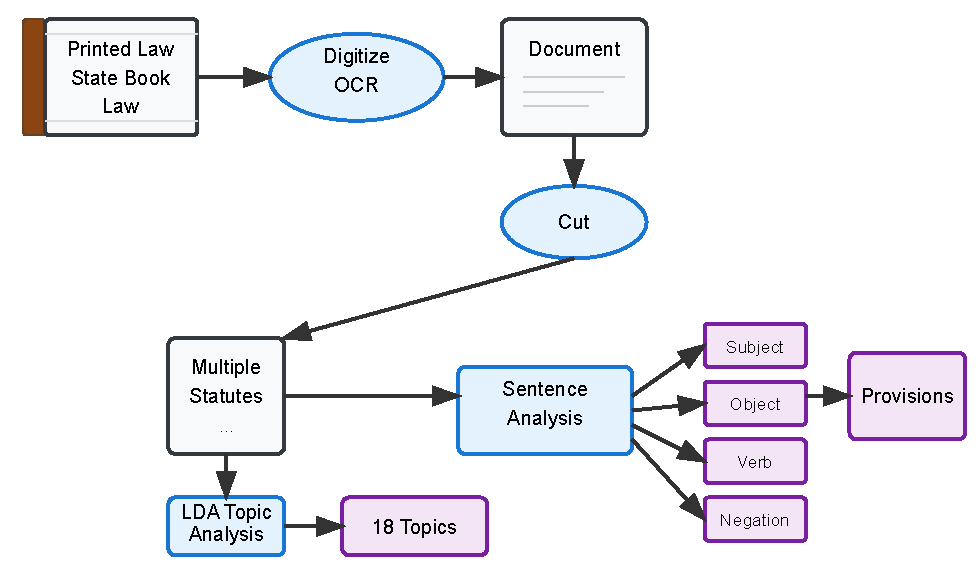
\includegraphics[width=\textwidth]{pic/fig4.pdf} % Use \textwidth to fill column
            \end{figure}
            \vfill
        \end{column}
    \end{columns}
\end{frame}

\section{Empirical Approach}
\begin{frame}
    \frametitle{Linear Regression Model}
    \footnotesize
    The paper specifies the following linear regression model:
    \begin{equation}
        \Delta \log Y_{st} = \alpha_s + \alpha_t + \alpha_s \cdot t + \rho \log W_{st} + X'_{st}\beta + \epsilon_{st}
    \end{equation}
    Where:
    \begin{itemize}
        \item $\Delta \log Y_{st}$: The log change in real per capita GDP in state $s$ during biennium $t$. This is the dependent variable representing economic growth.
        \item $W_{st}$: The number of legal provisions enacted in state $s$ during biennium $t$.
        \item $\alpha_s$: State fixed effects, capturing time-invariant characteristics specific to each state.
        \item $\alpha_t$: Time (biennium) fixed effects, accounting for common shocks or trends affecting all states in a particular biennium.
        \item $\alpha_s \cdot t$: State-specific time trends, allowing for different linear trends over time for each state.
        \item $X'_{st}$: A vector of additional covariates used for robustness checks.
    \end{itemize}
\end{frame}

\begin{frame}
    \frametitle{Shift-Share Instrument for Legislative Diffusion}
    \begin{itemize}
        \item The paper uses a shift-share instrument to address the potential endogeneity (reverse causality) of legislative diffusion.
        \item The instrument is constructed based on the idea that states tend to borrow laws rather than draft from scratch.
        \begin{itemize}
            \item \textbf{shifter}: nationwide growth in topic-specific legislating
            \item \textbf{shares}: a state's preperiod stock of legislative output on each topic
        \end{itemize}

    \end{itemize}   
\end{frame}

\begin{frame}
    \frametitle{Shift-Share Instrument for Legislative Diffusion}
    \footnotesize
    \begin{itemize}
            \item \textbf{shifter}: Nationwide growth in topic-specific legislating. Formally: $\frac{1}{49}\sum_{r \neq s}\Delta \log W_{rt}^k$
            \item \textbf{shares}: A state's preperiod stock of legislative output on each topic. Formally: $\frac{W_{s0}^k}{W_{s0}}$
    \end{itemize}
    \vspace{0.5em} % Add some vertical space
    The instrument is constructed as:
    \begin{equation}
        Z_{st} = \sum_{k=1}^{K} \underbrace{\frac{W_{s0}^k}{W_{s0}}}_{\text{shares}} \underbrace{\sum_{r \neq s} \frac{\Delta \log W_{rt}^k}{49}}_{\text{shifts}}
    \end{equation}
    The first-stage equation for legislative output is:
    \begin{equation}\label{first_stage}
        \log W_{st} = \alpha_s + \alpha_t + \alpha_s \cdot t + \psi Z_{st} + X'_{st}\beta + \eta_{st}
    \end{equation}
    Reduced-form estimates are produced by:
    \begin{equation}\label{reduced_form}
        \Delta \log Y_{st} = \alpha_s + \alpha_t + \alpha_s \cdot t + \gamma Z_{st} + X'_{st}\beta + \epsilon_{st}
    \end{equation}
\end{frame}

\begin{frame}
    \frametitle{First Stage Regression}
     \begin{equation*}
        \log W_{st} = \alpha_s + \alpha_t + \alpha_s \cdot t + \psi Z_{st} + X'_{st}\beta + \eta_{st}
        \tag{\ref{first_stage}}
    \end{equation*}
    \begin{itemize}
            \footnotesize
        \item In classic shift-share instruments (e.g., employment) having high previous shares of sectors that are increasing nationally will tend to get pulled upward.
        \item In this paper, the effect of $Z_{st}$ however, is \textbf{negative}, as states having lower previous shares of topics will be more likely to increase to national trends.
    \end{itemize}
    \begin{figure}[htbp]
        \centering
        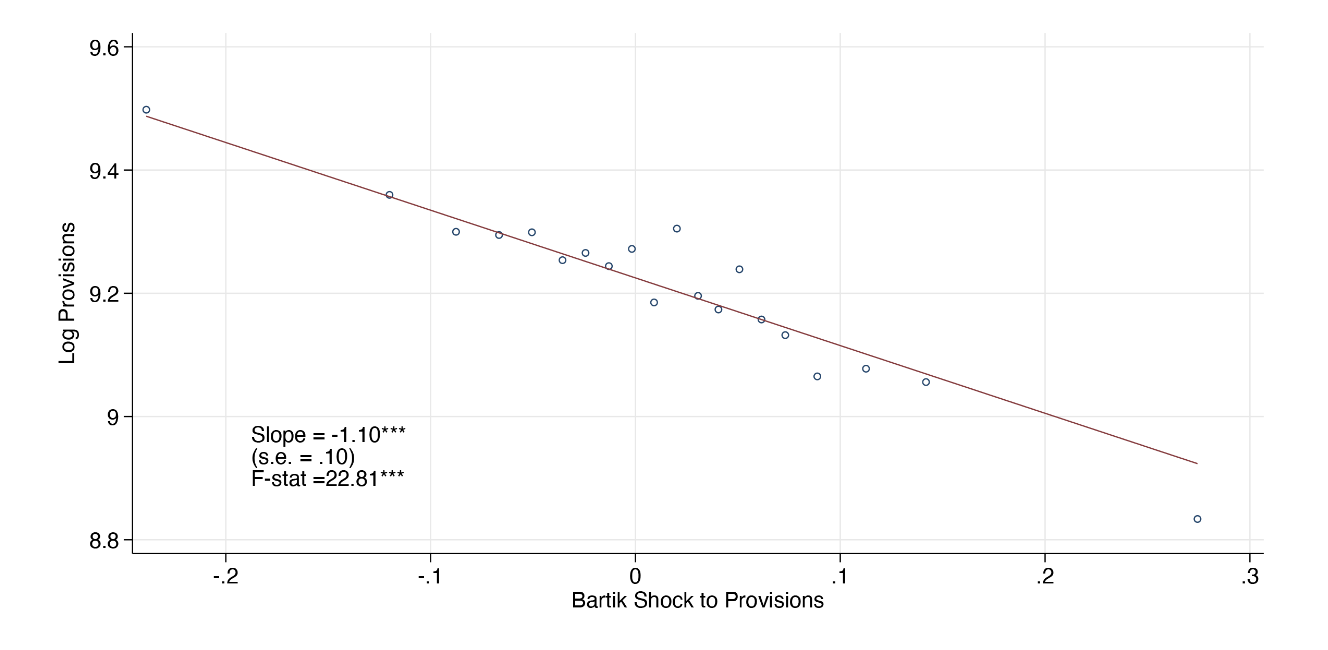
\includegraphics[width=0.7\textwidth]{pic/fig5.png}
        \captionsetup{font=footnotesize}
    \end{figure}
\end{frame}

\begin{frame}
    \frametitle{Exogeneity and Exclusion}
    \footnotesize
    \begin{itemize}
        \item \textbf{Approach 1: Conditional Exogeneity of Preperiod Shares}
        \begin{itemize}
            \item Assumes preperiod topic \textbf{shares} are not related with economic growth afterwards.
        \end{itemize}
    \end{itemize}
    \begin{figure}[htdp]
        \centering
        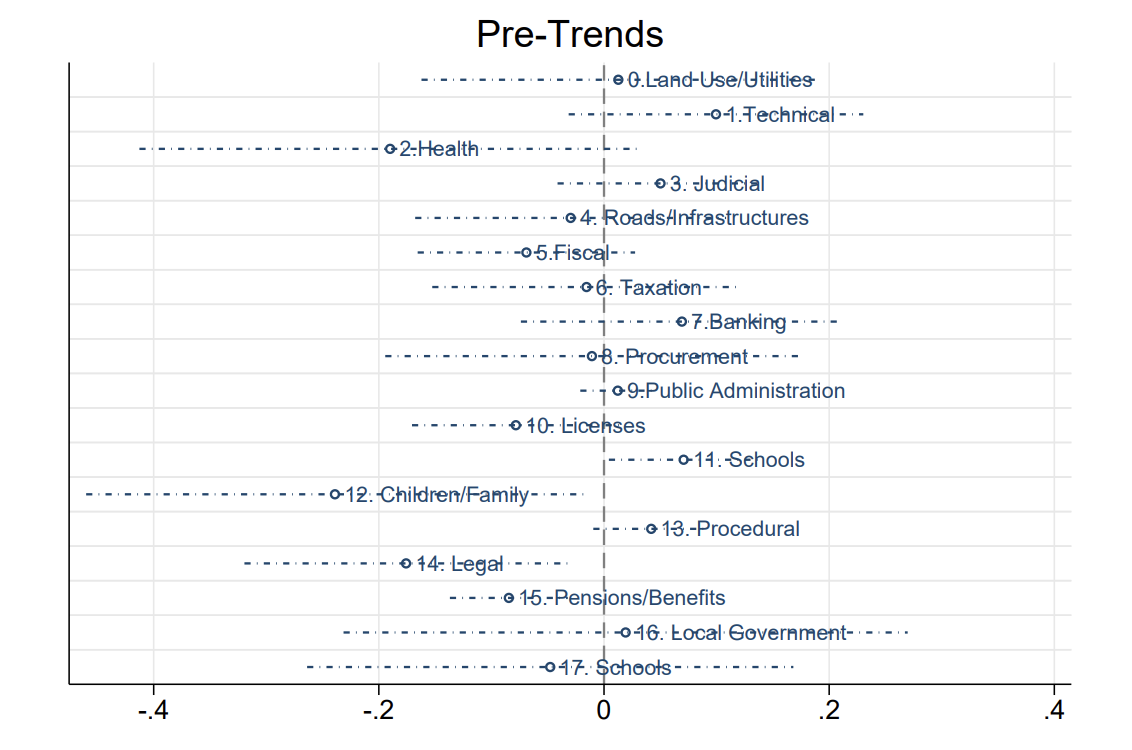
\includegraphics[width=0.7\textwidth]{pic/fig6.png}
    \end{figure}
\end{frame}

\begin{frame}
    \frametitle{Exogeneity and Exclusion}
    \footnotesize
    \begin{itemize}
        \item \textbf{Approach 2: Conditional Exogeneity of Current-Period Shifters}
        \begin{itemize}
            \item Assumes global shocks (shifters) are uncorrelated with exposure-weighted average of potential outcomes (conditional on fixed effects, controls, and state-time trends).
            \item \textit{Validation Checks:}
            \begin{itemize}
                \item \textbf {Relevance test议题相关性检验}: Instrument relevance driven by a majority of topics.
                \item \textbf {Weak instrument test弱工具变量检验} (Olea and Pflueger 2013): Effective F-statistic = 132.8 (strong).
                \item \textbf {Placebo test安慰剂检验}: Economic growth not correlated with future instrument values (Table A.12).
                \item \textbf {Balance test混淆变量检验}: Instrument not correlated with current/lagged state characteristics (Table A.14).
            \end{itemize}
        \end{itemize}
    \end{itemize}
\end{frame}

\section{Main Results}

\begin{frame}
    \frametitle{Main Regression Results}
    \begin{table}[c] % Use [c] for centering in beamer, or omit
        \centering
        \caption{First Stage (FS), OLS, and Reduced Form (RF) Estimates}
        \label{tab:main_results}
        \resizebox{\textwidth}{!}{% Resize table to fit slide width
        \begin{tabular}{@{}lcccccc@{}}
            \toprule
            & \multicolumn{2}{c}{Effect on Provisions} & \multicolumn{4}{c}{Effect on Real GDP Growth per Capita} \\
            \cmidrule(lr){2-3} \cmidrule(lr){4-7}
            & FS & FS & OLS & OLS & RF & RF \\
            & (1) & (2) & (3) & (4) & (5) & (6) \\
            \midrule
            Legislative output & & & 0.0146* & 0.0152 & & \\
            & & & (0.00832) & (0.0123) & & \\
            \addlinespace
            Instrument ($Z_{st}$) & -1.099*** & -1.221*** & & & -0.0200** & -0.0205** \\
            & (0.230) & (0.259) & & & (0.00883) & (0.00940) \\
            \addlinespace
            Observations & 1,183 & 1,183 & 1,182 & 1,182 & 1,182 & 1,182 \\
            $R^2$ & 0.813 & .9 & 0.431 & 0.446 & 0.420 & 0.440 \\
            \addlinespace
            State fixed effects & X & X & X & X & X & X \\
            Time fixed effects & X & X & X & X & X & X \\
            State-specific trends & & X & & X & & X \\
            \bottomrule
            \multicolumn{7}{@{}p{\dimexpr\linewidth-2\tabcolsep\relax}@{}}{%
                \footnotesize \textit{Note:} Table shows OLS estimates. Standard errors are in parentheses. 
                
                Significance levels: * $p<.10$, ** $p<.05$, *** $p<.01$.

            } \\
        \end{tabular}%
        }
    \end{table}
%一阶段显著为负,初期立法量越低,后期显著高;OLS直接回归显示无直接影响,表明存在潜在的内生性问题;直接用工具变量回归显示,初期立法量越低,后期GDP增长显著高。
\end{frame}
\begin{frame}
    \frametitle{Main Regression Results (2SLS)}
\begin{table}[c]
        \centering
        \caption{Effect of Legislative Output on Economic Growth (2SLS)}
        \label{tab:2sls_results}
        \resizebox{\textwidth}{!}{%
        \begin{tabular}{@{}lccccccc@{}}
            \toprule
            & \multicolumn{7}{c}{Effect on Growth Rate per Capita} \\
            \cmidrule(lr){2-8}
            & (1) & (2) & (3) & (4) & (5) & (6) & (7) \\
            \midrule
            Legislative output & .0182** & .0168* & .0152** & .0134* & .0116* & .0222** & .0094* \\
            & (.00903) & (.00863) & (.00704) & (.00687) & (.00602) & (.0106) & (.00507) \\
            \addlinespace
            First-stage \textit{F}-statistic & 22.86  & 22.19  & 23.11  & 22.92  & 44.51  & 19.69  & 27.30  \\
            Observations         & 1,182  & 1,182  & 1,182  & 1,182  & 1,134  & 1,182  & 1,086  \\
            \addlinespace
            Time fixed effects   & X      & X      & X      & X      & X      & X      & X      \\
            State fixed effects  & X      & X      & X      & X      & X      & X      & X      \\
            State trends         &        & X      &        &        &        &        & X      \\
            \addlinespace
            Economic variables $\times$ time & & & X & & & & X \\
            Sector shares $\times$ time      & & & & X & & & X \\
            Demographic variables $\times$ time& & & & & X & & X \\
            Topic shares                     & & & & & & X & X \\
            Lagged government expenditures   & & & & & & & X \\
            Lagged dependent variable        & & & & & & & X \\
            \bottomrule
            \multicolumn{8}{@{}p{\dimexpr\linewidth-2\tabcolsep\relax}@{}}{%
                \footnotesize \textit{Note:} Table shows 2SLS estimates. Standard errors are in parentheses. 

                Significance levels: * $p<.10$, ** $p<.05$, *** $p<.01$.

                            } \\
        \end{tabular}%
        }
    \end{table}
\end{frame}

\begin{frame}
    \frametitle{Robustness Checks}
    \begin{itemize}
        \item Leads and Lags Analysis
        \item Topic-Related Checks
        \item Alternative Measures of Legislative Detail
        \item Alternative Outcomes
        \begin{itemize}
            \item GDP growth
            \item Profits
            \item Labor income
        \end{itemize}
        \item Checks on Other Government Activities
        \item Investigation of Alternative Legal Sources
        \item Alternative Clustering of Standard Errors 
    \end{itemize}
\end{frame}
\section{Additional Analyses}

\begin{frame}
    \frametitle{Mechanisms:Framework}
    \footnotesize
    The conceptual framework is based on the \textbf{holdup model}:
    \begin{itemize}
        \item \textbf{Core Idea:} More complete legislation can increase location- and relationship-specific investments by reducing the risk of ex post holdup.
        \item \textbf{Mechanism for Growth:} Increased completeness in legislation reduces uncertainty, encouraging fuller investment and thereby promoting economic growth.
      
    \end{itemize}
\end{frame}

\begin{frame}
    \frametitle{Mechanisms:Framework}
    \footnotesize
    \begin{itemize}
         \item \textbf{Additional Predictions:}
        \begin{itemize}
        \item \textbf{Policy Topics:} Effects are expected to be stronger for laws regulating business compared to other policy areas.
        \item \textbf{Contingent Clauses:} Clauses that specify actions based on the state of the world (contingencies) are predicted to be more effective in promoting growth, as they reduce ambiguity.
        \item \textbf{Concavity in Existing Legal Detail:} The marginal benefit of additional legal clauses is expected to be higher in areas with initially less legal detail (concavity).
        \item \textbf{Relationship Specificity:} Growth effects of laws should be more pronounced in sectors relying heavily on relationship-specific inputs.
        \item \textbf{Economic Policy Uncertainty (EPU):} The positive impact of increased legal detail (especially contingent clauses) on growth is expected to be larger when EPU is high.
        \end{itemize}
    \end{itemize}
\end{frame}

\begin{frame}
    \frametitle{Mechanisms:Policy Topics}
    \begin{table}[htdp]
        \centering
        \caption{What Policies Are Driving the Effect of Lawmaking on Growth?}
        \label{tab:policies_growth}
        \resizebox{\textwidth}{!}{%
        \begin{tabular}{@{}lcccc@{}}
            \toprule
            & \multicolumn{4}{c}{EFFECT ON REAL GDP GROWTH PER CAPITA} \\
            \cmidrule(lr){2-5}
            POLICY CATEGORY & Economic Regulation & Social Regulation & Fiscal & Procedural \\
            & (1) & (2) & (3) & (4) \\
            \midrule
            Legislative output & .0125* & -.0006 & .0220** & .0009 \\
            & (.00697) & (.0097) & (.0107) & (.009) \\
            \addlinespace
            First-stage $F$-statistic & 42.53 & 13.42 & 18.68 & 49.12 \\
            Observations & 1,182 & 1,182 & 1,181 & 1,182 \\
            Time fixed effects & X & X & X & X \\
            State fixed effects & X & X & X & X \\
            \bottomrule
            \multicolumn{5}{@{}p{\dimexpr\linewidth-2\tabcolsep\relax}@{}}{%
                \footnotesize \textit{Note:} Significance levels: * $p<.10$, ** $p<.05$.
            } \\
        \end{tabular}%
        }
    \end{table}
\end{frame}

\begin{frame}
    \frametitle{Mechanisms:Contingent Clauses}
    \footnotesize
    \begin{itemize}
        \item \textbf{Analyses of Contingency:} Research applied a contingency dictionary to divide the corpus into two parts: contingent provisions ($W_{st}^C$) and noncontingent provisions ($W_{st}^N$).
        \item \textbf{Model with Joint Endogenous Regressors:}
        \begin{itemize}
            \item The second stage is:
            \begin{equation*}
                \Delta \log Y_{st} = \alpha_s + \alpha_t + \alpha_s \cdot t + \rho_C \log W_{st}^C + \rho_N \log W_{st}^N + X'_{st}\beta + \epsilon_{st}
            \end{equation*}
            \item Two instruments are used, $Z_{st}^C$ (contingency instrument) and $Z_{st}^N$ (non-contingency instrument). The first-stage equations are:
            \begin{align*}
                \log W_{st}^C &= \alpha_s + \alpha_t + \alpha_s \cdot t + \psi_C Z_{st}^C + \psi_N Z_{st}^N + X'_{st}\beta + \eta_{st}^C \\
                \log W_{st}^N &= \alpha_s + \alpha_t + \alpha_s \cdot t + \psi_C Z_{st}^C + \psi_N Z_{st}^N + X'_{st}\beta + \eta_{st}^N
            \end{align*}
        \end{itemize}
    \end{itemize}
\end{frame}

\begin{frame}
    \frametitle{Mechanisms:Contingent Clauses}
    \footnotesize
    \begin{itemize}
        \item \textbf{Analyses of Contingency:} Research applied a contingency dictionary to divide the corpus into two parts: contingent provisions ($W_{st}^C$) and noncontingent provisions ($W_{st}^N$).
   \item \textbf{Alternative Specification (Log Difference):}
        \begin{itemize}
            \item The second stage, with $\log W_{st}^C - \log W_{st}^N$ as a single endogenous regressor:
            \begin{equation*}
                \Delta \log Y_{st} = \alpha_s + \alpha_t + \alpha_s \cdot t + \rho_{CN} (\log W_{st}^C - \log W_{st}^N) + X'_{st}\beta + \epsilon_{st}
            \end{equation*}
            \item The first stage for this specification:
            \begin{equation*}
                (\log W_{st}^C - \log W_{st}^N) = \alpha_s + \alpha_t + \alpha_s \cdot t + \psi_C Z_{st}^C + \psi_N Z_{st}^N + X'_{st}\beta + \eta_{st}
            \end{equation*}
        \end{itemize}
    \end{itemize}
\end{frame}


\begin{frame}
    \frametitle{Mechanisms:Contingent Clauses}
    \begin{table}[h!]
        \centering
        \caption{Effect of Contingent and Noncontingent Clauses on Economic Growth}
        \label{tab:contingent_clauses_growth}
        \resizebox{\textwidth}{!}{%
        \begin{tabular}{@{}lccccccc@{}}
            \toprule
            & \multicolumn{7}{c}{EFFECT ON REAL GDP GROWTH PER CAPITA} \\
            \cmidrule(lr){2-8}
            & (1) & (2) & (3) & (4) & (5) & (6) & (7) \\
            \midrule
            Contingent provisions & .0638*** & .0590*** &  &  &  &  &  \\
            & (.0226) & (.0215) &  &  &  &  &  \\
            \addlinespace
            Noncontingent provisions & -.0559** & -.0511** &  &  &  &  &  \\
            & (.0242) & (.0228) &  &  &  &  &  \\
            \addlinespace
            Contingent $-$ noncontingent &  &  & .0752*** & .0697*** & .0501** & .0379** & .0773*** \\
            &  &  & (.0242) & (.0229) & (.0219) & (.0158) & (.0219) \\
            \addlinespace
            First-stage $F$-statistic & 22.27 & 36.82 & 22.83 & 36.60 & 15.13 & 31.68 & 23.86 \\
            Observations & 1,182 & 1,182 & 1,182 & 1,182 & 1,182 & 1,182 & 1,134 \\
            \addlinespace
            Time fixed effects & X & X & X & X & X & X & X \\
            State fixed effects & X & X & X & X & X & X & X \\
            State trends &  & X &  & X &  &  &  \\
            \addlinespace
            Economic variables $\times$ time &  &  &  &  & X &  &  \\
            Sector shares $\times$ time &  &  &  &  &  & X &  \\
            Demographic variables $\times$ time &  &  &  &  &  &  & X \\
            \bottomrule
            \multicolumn{8}{@{}p{\dimexpr\linewidth-2\tabcolsep\relax}@{}}{%
                \footnotesize \textit{Note:} Significance levels: * $p<.10$, ** $p<.05$, *** $p<.01$. 
            } \\
        \end{tabular}%
        }
    \end{table}
\end{frame}

\begin{frame}
    \frametitle{Mechanisms:Concavity in Existing Legal Detail}
    \begin{table}[h!]
        \centering
        \caption{Concavity: Effect of Provisions on Growth by Recent Detail Level}
        \label{tab:concavity_growth}
        \resizebox{\textwidth}{!}{%
        \begin{tabular}{@{}lccccccc@{}}
            \toprule
            & \multicolumn{7}{c}{Effect on Real GDP Growth Per Capita} \\
            \cmidrule(lr){2-8}
            Recent Legal Detail & \multicolumn{3}{c}{Low} & \multicolumn{2}{c}{Medium} & \multicolumn{2}{c}{High} \\
            \cmidrule(lr){2-4} \cmidrule(lr){5-6} \cmidrule(lr){7-8}
            & (1) & (2) & (3) & (4) & (5) & (6) & (7) \\
            \midrule
            Legislative Output & 0.0404* & 0.0425* & & 0.00640 & 0.000205 & 0.0002 & -0.0109 \\
            & (0.0167) & (0.0158) & & (0.0104) & (0.0107) & (0.00743) & (0.00935) \\
            \addlinespace
            Contingent - & & & 0.117** & & & & \\
            Non-Contingent & & & (0.0351) & & & & \\
            \midrule
            First Stage F-stat & 66.18 & 59.26 & 25.29 & 48.65 & 47.87 & 86.59 & 67.12 \\
            Observations & 392 & 392 & 392 & 385 & 385 & 382 & 382 \\
            \addlinespace
            Time FE & X & X & X & X & X & X & X \\
            State FE & X & X & X & X & X & X & X \\
            State Trends & & X & X & & X & & X \\
            \bottomrule
            \multicolumn{8}{@{}p{\dimexpr\linewidth-2\tabcolsep\relax}@{}}{%
                \footnotesize \textit{Note:} Significance levels: * $p<.10$, ** $p<.05$.
            } \\
        \end{tabular}%
        }
    \end{table}
\end{frame}

\begin{frame}
    \frametitle{Mechanisms:Sectoral Relationship Specificity}
\begin{table}[h]
  \centering
  \caption{Heterogeneous Effects by Relationship-Specific Investments}
  \resizebox{\textwidth}{!}{%
  \begin{tabular}{lccccccccc}
    \toprule
    & \multicolumn{9}{c}{Effect on Real GDP Growth by Sector Group} \\
    \cmidrule(lr){2-10}
    & \multicolumn{3}{c}{Low Relationship Specificity} & \multicolumn{6}{c}{High Relationship Specificity} \\
    \cmidrule(lr){2-4} \cmidrule(lr){5-10}
    & (1) & (2) & (3) & (4) & (5) & (6) & (7) & (8) & (9) \\
    \midrule
    Legislative output & .000231 & & & .0488** & .0414* & & & & \\
    & (.0221) & & & (.0225) & (.0211) & & & & \\
    \addlinespace
    Contingent provisions & & $-.00659$ & & & & .217* & .177* & & \\
    & & (.0979) & & & & (.109) & (.104) & & \\
    \addlinespace
    Noncontingent provisions & & .00864 & & & & $-.204*$ & $-.164$ & & \\
    & & (.117) & & & & (.117) & (.113) & & \\
    \addlinespace
    Contingent $-$ noncontingent & & & $-.00342$ & & & & & .237** & .197** \\
    & & & (.0795) & & & & & (.103) & (.0952) \\
    \midrule
    First-stage $F$-statistic & 22.83 & 18.2 & 19.26 & 22.83 & 21.74 & 18.2 & 34.4 & 19.26 & 33.42 \\
    Observations & 1,133 & 1,133 & 1,133 & 1,133 & 1,133 & 1,133 & 1,133 & 1,133 & 1,133 \\
    Time fixed effects & X & X & X & X & X & X & X & X & X \\
    State fixed effects & X & X & X & X & X & X & X & X & X \\
    State trends & & & & & X & & X & & X \\
    \bottomrule
    \multicolumn{10}{l}{} \\
  \end{tabular}%
  }
  \label{tab:heterogeneous_effects}%
\end{table}
\end{frame}

\begin{frame}
    \frametitle{Mechanisms:Economic Policy Uncertainty (EPU)}
    \begin{table}[htbp]
  \centering
  \caption{Effect of Laws on Growth by the Level of EPU}
  \resizebox{\textwidth}{!}{%
  \begin{tabular}{lcccccccccc}
    \toprule
    & \multicolumn{10}{c}{Effect on Real GDP Growth Per Capita} \\
    \cmidrule(lr){2-11}
    & \multicolumn{2}{c}{Low Economic} & \multicolumn{2}{c}{Medium Economic} & \multicolumn{6}{c}{High Economic Uncertainty} \\
    & \multicolumn{2}{c}{Uncertainty} & \multicolumn{2}{c}{Uncertainty} & \multicolumn{6}{c}{} \\
    \cmidrule(lr){2-3} \cmidrule(lr){4-5} \cmidrule(lr){6-11}
    & (1) & (2) & (3) & (4) & (5) & (6) & (7) & (8) & (9) & (10) \\
    \midrule
    Legislative output & .00448 & & .00699 & & .0373** & .0391** & & & & \\
    & (.0111) & & (.0111) & & (.0153) & (.0176) & & & & \\
    \addlinespace
    Contingent provisions & & & & & & & .145** & .170** & & \\
    & & & & & & & (.0560) & (.0672) & & \\
    \addlinespace
    Noncontingent provisions & & & & & & & $-.137**$ & $-.163**$ & & \\
    & & & & & & & (.0624) & (.0775) & & \\
    \addlinespace
    Contingent $-$ noncontingent & & .0823 & & .000182 & & & & & .164*** & .189*** \\
    & & (.0692) & & (.0310) & & & & & (.0465) & (.0568) \\
    \midrule
    First-stage $F$-statistic & 65.92 & 4.251 & 5.389 & 12.03 & 46.50 & 108.2 & 10.24 & 9.433 & 10.65 & 10.34 \\
    Observations & 345 & 345 & 373 & 373 & 377 & 377 & 377 & 377 & 377 & 377 \\
    Time fixed effects & X & X & X & X & X & X & X & X & X & X \\
    State fixed effects & X & X & X & X & X & X & X & X & X & X \\
    State trends & & & & & & X & & X & & X \\
    \bottomrule
    \multicolumn{11}{l}{\footnotesize Standard errors in parentheses. ** $p<0.05$, *** $p<0.01$ (assumed).} \\
  \end{tabular}%
  }
  \label{tab:epu_effects}%
\end{table}
\end{frame}

\section{Conclusion}

\begin{frame}
    \footnotesize
    \frametitle{Conclusion}
    \begin{columns}[T]
        \begin{column}{0.5\textwidth}
            \textbf{Key Findings}
            \begin{itemize}
                \item More legislation tends to boost economic growth
                \item Impact is driven by \textit{economic} rather than social regulations
                \item Effect is stronger for:
                \begin{itemize}
                        \footnotesize
                    \item Contingent clauses (vs. non-contingent)
                    \item Sectors with high relationship-specificity
                    \item States with lower initial legislative detail
                    \item Periods of greater economic policy uncertainty
                \end{itemize}
            \end{itemize}
        \end{column}
        \begin{column}{0.5\textwidth}
            \textbf{Methodological Contributions}
            \begin{itemize}
                \item Novel use of legal text data in causal framework
                \item New measure of legislative output using computational linguistics
                \item Text-based shift-share instrumental variables strategy
            \end{itemize}
            
            \vspace{0.5em}
            \textbf{Future Directions}
            \begin{itemize}
                \item Explore spillover effects on neighboring states
                \item Test external validity in other federal systems
                \item Examine varying institutional frameworks
            \end{itemize}
        \end{column}
    \end{columns}
\end{frame}

\begin{frame}
\Background
    \frametitle{}
    \begin{center} 
        \Huge 
        \emph{Thank You!}
    \end{center}

    \vspace{1em}
    \begin{center}
        \large
    2025-05-20
    \end{center}
    \vspace{1em}
\end{frame}
\end{document}